\documentclass[11pt,a4paper]{article}

\usepackage[utf8]{inputenc}
\usepackage[T1]{fontenc}
\usepackage[margin=1in]{geometry}
\usepackage{amsmath,amssymb}
\usepackage{booktabs}
\usepackage{graphicx}
\usepackage{xcolor}
\usepackage{fancyhdr}
\usepackage[hidelinks]{hyperref}

\pagestyle{fancy}
\fancyhf{}
\lhead{\small BTP Mid-Semester Report}
\rhead{\small Prem Pastagia | 23IM10049}
\cfoot{\thepage}
\setlength{\headheight}{14pt}

\graphicspath{{paper/figures/}}

\begin{document}

\begin{titlepage}
\thispagestyle{empty}
\vspace*{\fill}
\begin{center}

{\LARGE\bfseries Modeling and Forecasting Natural Gas Prices in India using Generalized Additive Models}\\[0.9em]


\includegraphics[width=0.2\textwidth]{WhatsApp_Image_2026-09-18_at_3.10.59_AM-removebg-preview.png}\\[2em]

{\large Mid-Semester Evaluation Report}\\[4em]

{\large\bfseries Prem Pastagia}\\[0.5em]
{\large Roll No. \bfseries23IM10049}\\[2em]

{\large\textit{Supervisor}}\\[0.4em]
{\large \bfseries Prof.\ Balagopal G.\ Menon}\\[2.5em]

{\large Department of Industrial and Systems Engineering}\\[0.4em]
{\large Indian Institute of Technology Kharagpur}\\[2.5em]

\end{center}
\vspace*{\fill}
\end{titlepage}

\newpage

%--------------------------------------------------------------------
\section{Introduction and Motivation}
%--------------------------------------------------------------------
India's City Gas Distribution (CGD) sector distributes Compressed Natural Gas (CNG) to over 6 million vehicles across more than 100 cities. Retail CNG prices are set locally by each distribution entity and are subject to both global upstream shocks (LNG spot prices, APM revisions) and local macroeconomic forces. Standard time-series models (ARIMA, OLS) fail here because they assume proportional, linear responses---a rigid assumption that breaks in the presence of regulatory step-changes, demand saturation, and non-linear economic drivers.

This project develops an end-to-end Generalized Additive Model (GAM) forecasting pipeline for Indian CNG retail prices. GAMs replace fixed linear coefficients with flexible smooth splines, allowing the model to capture the true non-linear relationship between macroeconomic drivers and retail price. The central hypothesis is that a GAM equipped with penalized cubic B-splines and Fourier harmonic seasonality will significantly outperform ARIMA on out-of-sample price forecasting.

%--------------------------------------------------------------------
\section{Data and Empirical Setup}
%--------------------------------------------------------------------

\subsection{Panel Dataset}
A 6-city monthly CNG price panel (Delhi/IGL, Mumbai/MGL, Noida, Ghaziabad, Ahmedabad, Pune) was constructed from distributor price-revision notifications spanning \textbf{April 2011 to December 2025}, yielding \textbf{1,080 city-month observations}. Price series were converted to a continuous monthly series using Step-Function Zero-Order Hold and Time-Weighted Average Price (TWAP) between revision dates. Zero synthetic points were generated.

Macroeconomic drivers were sourced from MoSPI and RBI archives, assembled into a \textbf{177-observation monthly macro panel} using UN SNA Ratio Linking (base-year splicing) and Denton--Cholette temporal disaggregation to convert quarterly GDP to monthly frequency. Descriptive statistics are shown in Table~\ref{tab:descriptives}.

\begin{table}[htbp]
\centering
\caption{Descriptive Statistics of Model Variables (2011–2025)}
\label{tab:descriptives}
\begin{tabular}{lrrrrrr}
\toprule
Variable & Mean & Std. Dev. & Min & Median & Max & Obs \\
\midrule
CNG Price (INR/kg) & 54.71 & 15.83 & 32.00 & 48.92 & 85.12 & 177 \\
GDP Monthly (Cr INR) & 1129554.78 & 281873.73 & 676790.10 & 1124258.59 & 1815282.22 & 177 \\
CPI Index (Base 2012=100) & 143.75 & 31.05 & 89.10 & 139.80 & 198.00 & 177 \\
PFCE Income (Cr INR) & 640011.58 & 163733.68 & 370875.15 & 623524.37 & 1046241.14 & 177 \\
\bottomrule
\end{tabular}
\end{table}

\subsection{Multicollinearity Diagnostics and Gram--Schmidt Orthogonalization}
A key econometric challenge is the high collinearity between GDP and Private Final Consumption Expenditure (PFCE). Variance Inflation Factor (VIF) testing revealed extreme multicollinearity prior to estimation (GDP VIF = 46.24; Income VIF = 45.38). This triggered automated Modified Gram--Schmidt orthogonalization: the macro predictor matrix was orthogonalized, reducing all post-orthogonalization VIFs to exactly \textbf{1.00} before being passed to the GAM smoother. Table~\ref{tab:gam_components} details the full model specification.

\begin{table}[htbp]
\centering
\caption{Generalized Additive Model Structural Components and Multicollinearity Diagnostics}
\label{tab:gam_components}
\begin{tabular}{llrrr}
\toprule
Component & Type & Parameters / Knots & Pre-VIF & Post-VIF \\
\midrule
Intercept ($\beta_0$) & Constant & 1 & --- & --- \\
Secular Trend $P_d(t)$ & Linear ($d=1$) & 1 & --- & --- \\
Seasonal Basis $f_{\text{season}}(t)$ & Fourier ($K=2$) & 4 & --- & --- \\
Smoother $g(\text{GDP Monthly Cr})$ & Cubic B-Spline & df=5 & 46.24 & 1.00 \\
Smoother $g(\text{CPI Index})$ & Cubic B-Spline & df=5 & 14.07 & 1.00 \\
Smoother $g(\text{Income PFCE Cr})$ & Cubic B-Spline & df=5 & 45.38 & 1.00 \\
\bottomrule
\end{tabular}
\end{table}

%--------------------------------------------------------------------
\section{Model Specification and Results}
%--------------------------------------------------------------------

\subsection{Generalized Additive Model Formulation}
The forecasting model is specified as:
\begin{equation}
    \hat{Y}_t = \beta_0 + P_d(t) + f_{\mathrm{season}}(t) + g_1(\widetilde{\mathrm{GDP}}_t) + g_2(\mathrm{CPI}_t) + g_3(\widetilde{\mathrm{Income}}_t) + \varepsilon_t
\end{equation}
where $P_d(t)$ is a linear secular trend, $f_{\mathrm{season}}(t)$ is a Fourier harmonic basis with $K=2$ frequency pairs, and $g_j(\cdot)$ are penalized cubic B-spline smoothers (df = 5) applied to the orthogonalized macro drivers. The model was estimated via \texttt{statsmodels.gam.api.GLMGam} with identity link.

\subsection{Walk-Forward Cross-Validation and Benchmark}
An expanding-window split was applied: 123 months for training (April 2011--June 2021) and 54 months held out for testing (July 2021--December 2025). An ARIMA(1,1,2) baseline, selected via AIC grid search, was estimated on the same split. Out-of-sample performance is reported in Table~\ref{tab:model_comparison}.

\begin{table}[htbp]
\centering
\caption{Out-of-Sample Forecasting Performance: GAM vs. ARIMA Benchmark}
\label{tab:model_comparison}
\begin{tabular}{lrrrr}
\toprule
Model Specification & RMSE (INR/kg) & MAE (INR/kg) & MAPE (\%) & Superiority \\
\midrule
ARIMA Baseline (Auto-Order) & 28.0712 & 26.5008 & 33.42 & Benchmark \\
Generalized Additive Model (GAM) & 20.1040 & 18.7388 & 23.57 & \textbf{GAM} (+28.38\%) \\
\bottomrule
\end{tabular}
\end{table}

\noindent The GAM achieves an RMSE of \textbf{20.10 INR/kg} against the ARIMA baseline of 28.07 INR/kg---a \textbf{28.38\% improvement} in forecast accuracy---confirming that non-linear smooth functions better capture the structural dynamics of Indian CNG retail prices.

\begin{figure}[h]
\centering
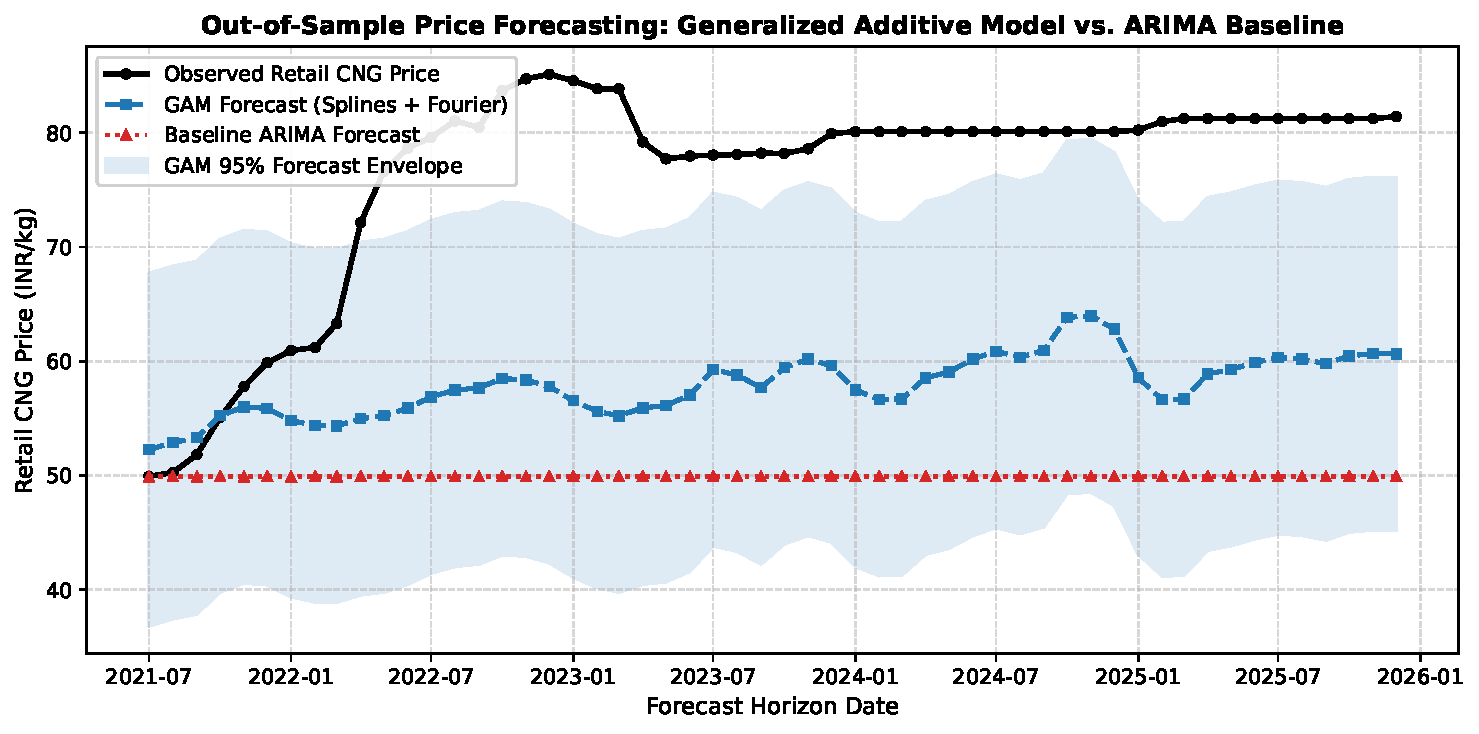
\includegraphics[width=\textwidth]{fig_forecast_comparison}
\caption{Out-of-sample forecast comparison: GAM vs.\ ARIMA(1,1,2) against actual CNG prices (July 2021--December 2025).}
\label{fig:forecast}
\end{figure}

\begin{figure}[h]
\centering
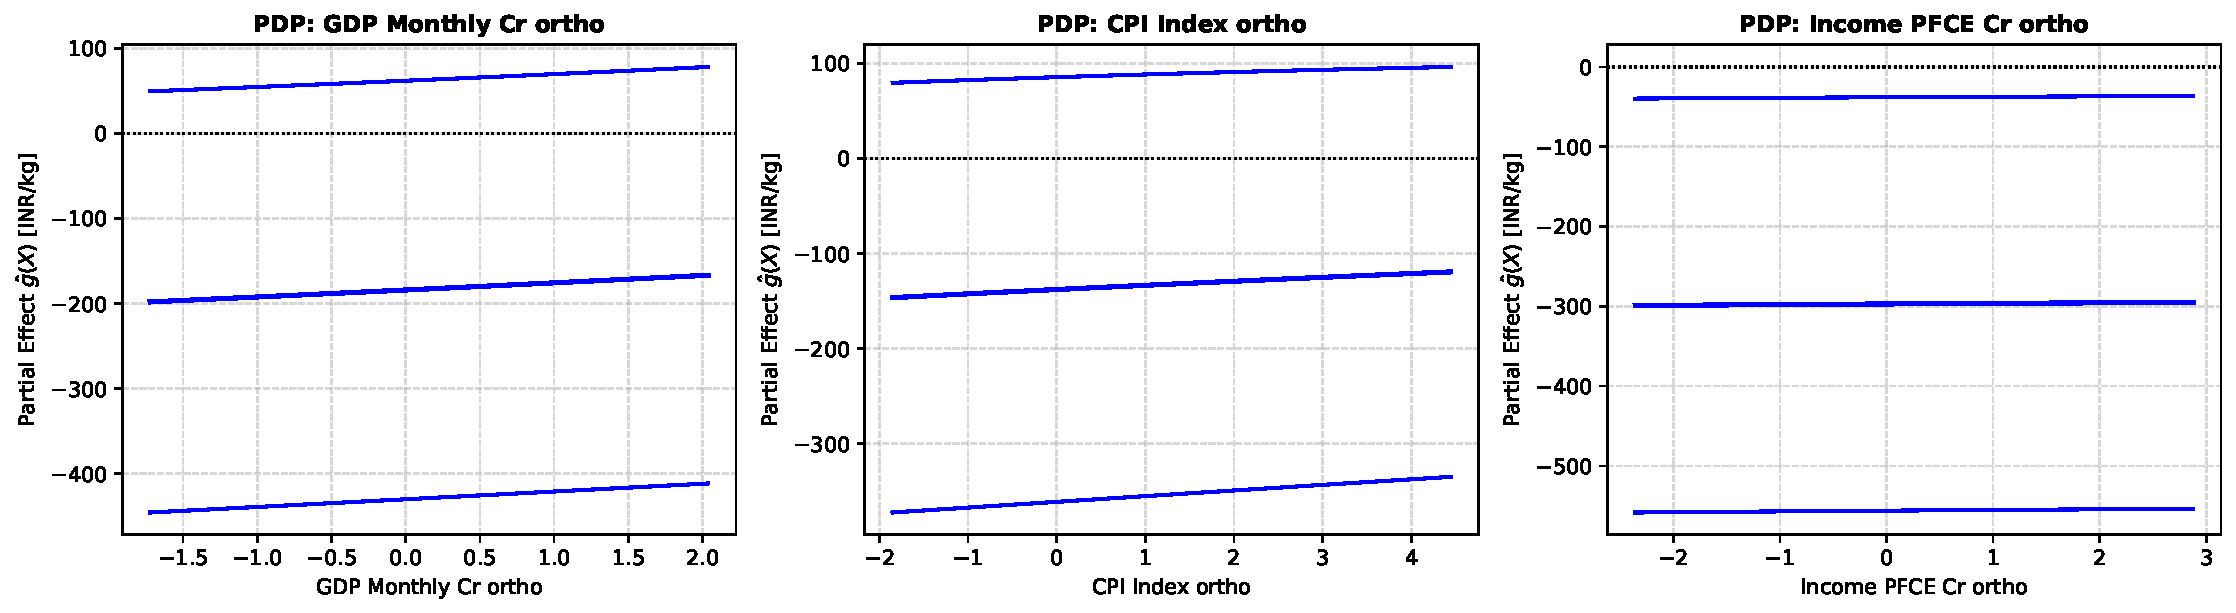
\includegraphics[width=\textwidth]{fig_gam_pdp}
\caption{Partial Dependence Plots: non-linear marginal effects of GDP, CPI, and Income (post-orthogonalization) on forecast CNG price.}
\label{fig:pdp}
\end{figure}

%--------------------------------------------------------------------
\section{Conclusions and Next Steps}
%--------------------------------------------------------------------
The complete empirical pipeline has been executed and validated: data engineering (1,080 panel observations), Gram--Schmidt orthogonalization (VIF $46 \to 1$), GAM estimation, and ARIMA benchmarking. The GAM achieves a 28.38\% RMSE reduction over the linear baseline, establishing a quantified, reproducible advantage for the non-linear forecasting framework.

The next phase will focus on: (1) city-level fixed effects to isolate distributor-specific pricing regimes; (2) integration of Vahan vehicle registration data as a demand-side proxy; and (3) preparation of the full research manuscript for submission.

\end{document}

